
\documentclass[aspectratio=169]{beamer}

%\usepackage[table]{xcolor}
\mode<presentation> {
\setbeamercovered{transparent}
  \usetheme{Boadilla}

%  \usetheme{Pittsburgh}
%\usefonttheme[2]{sans}
\renewcommand{\familydefault}{cmss}
%\usepackage{lmodern}
%\usepackage[T1]{fontenc}
%\usepackage{palatino}
%\usepackage{cmbright}
\usepackage{bm}
\usepackage{listings}
\useinnertheme{rectangles}
}



\usepackage{amsmath}
\usepackage{tcolorbox}
\setbeamercolor{normal text}{fg=black}
\setbeamercolor{structure}{fg= blue}
\definecolor{trial}{cmyk}{1,0,0, 0}
\definecolor{trial2}{cmyk}{0.00,0,1, 0}
\definecolor{darkgreen}{rgb}{0,.4, 0.1}
\usepackage{array}
\beamertemplatesolidbackgroundcolor{white}  \setbeamercolor{alerted
text}{fg=red}
\usepackage{tcolorbox}
\setbeamertemplate{caption}[numbered]\newcounter{mylastframe}

\font\domino=domino
\def\die#1{{\domino#1}}
\usepackage{tikz}
\usetikzlibrary{arrows}
\usetikzlibrary{arrows.meta, positioning}
\usepackage{colortbl}

\renewcommand{\familydefault}{cmss}
%\usepackage[all]{xy}

\usepackage{tikz}
\usepackage{lipsum}

 \newenvironment{changemargin}[3]{%
 \begin{list}{}{%
 \setlength{\topsep}{0pt}%
 \setlength{\leftmargin}{#1}%
 \setlength{\rightmargin}{#2}%
 \setlength{\topmargin}{#3}%
 \setlength{\listparindent}{\parindent}%
 \setlength{\itemindent}{\parindent}%
 \setlength{\parsep}{\parskip}%
 }%
\item[]}{\end{list}}
\usetikzlibrary{arrows}

\usecolortheme{lily}

\newtheorem{com}{Comment}
\newtheorem{lem} {Lemma}
\newtheorem{prop}{Proposition}
\newtheorem{condition}{Condition}
\newtheorem{thm}{Theorem}
\newtheorem{defn}{Definition}
\newtheorem{cor}{Corollary}
\newtheorem{obs}{Observation}
 \numberwithin{equation}{section}
 
\makeatletter
\def\beamerorig@set@color{%
  \pdfliteral{\current@color}%
  \aftergroup\reset@color
}
\def\beamerorig@reset@color{\pdfliteral{\current@color}}
\makeatother
\setbeamertemplate{navigation symbols}{}

\useoutertheme{miniframes}
\title[PLSC 30700]{Linear Models Lecture 13: IV}

\author{Robert Gulotty}
\institute[Chicago]{University of Chicago}
\vspace{0.3in}


\begin{document}

\begin{frame}
\maketitle
\end{frame}

\begin{frame}{2SLS and IV}
\begin{itemize}
\item IV formula:
 $$\hat{\beta}_{IV}=(Z'X)^{-1}Z'y$$
\item Two stage least squares:
\begin{itemize}
\item Suppose in the first stage we regress 
$$X=Z\gamma+v$$
\item In the second stage, we use $\hat{X}=Z\hat{\gamma}=Z(Z'Z)^{-1}Z'X=P_ZX$,
$$\hat{\beta}_{2SLS}=(\hat{X}'\hat{X})^{-1}\hat{X}'y$$
\end{itemize}
\item iv\_robust(Y $\sim$ $D + X | Z + X$, data = dat)
\end{itemize}
\end{frame}


\begin{frame}{Equivalence Between 2SLS and IV}
\begin{itemize}
\item 2SLS is exactly identical to IV when $l=k$
\begin{align*}
\hat{\beta}_{2SLS}&=(\hat{X}'\hat{X})^{-1}\hat{X}'y\\
&=(X'Z(Z'Z)^{-1}Z'X)^{-1}X'Z(Z'Z)^{-1}Z'y\\
&=(Z'X)^{-1}(Z'Z)(X'Z)^{-1}X'Z(Z'Z)^{-1}Z'y \tag{$(ABC)^{-1}=C^{-1}B^{-1}A^{-1}$}\\
&=(Z'X)^{-1}(Z'Z)(Z'Z)^{-1}Z'y\\
&=(Z'X)^{-1}Z'y=\hat{\beta}_{IV}
\end{align*}
\end{itemize}
\end{frame}


\section{Control Function}

\begin{frame}{Control Function Regression}
\begin{itemize}
\item Assume that $X_2$ is endogenous:
$$Y=\bm{x}_1'\beta_1+\bm{x}_2'\beta_2+e$$
$$\bm{x}_2=\Gamma'_{12}\bm{z}_1+\Gamma'_{22}\bm{z}_2+u_2$$
\item The control function approach directly models the error:
$$e=u_2'\alpha+v$$
$$\alpha=(E[u_2u_2'])^{-1}E[u_2e]$$
$$E[u_2v]=0$$
\end{itemize}
\end{frame}


\begin{frame}{Control Function Regression}
\begin{itemize}

\item We then plug this in to the original structural form equation, controlling for the error.
\begin{align*}
Y&=X_1'\beta_1+X_2'\beta_2+e\\
Y&=X_1'\beta_1+X_2'\beta_2+u_2'\alpha+v\\
E[X_1v]&=0\\
E[X_2v]&=0\\
E[u_2v]&=0
\end{align*}
\item After we control for $u_2$, the error is uncorrelated with X.
\item We estimate this new control with the reduced form residual:
$$\hat{u}_{2i}=\bm{x}_{2i}-\hat{\Gamma}'_{12}\bm{z}_1+\hat{\Gamma}'_{22}\bm{z}_2$$
\item It is like subtracting off the endogenous part.
$$\bm{Y}=\bm{X}\hat{\beta}+\bm{\hat{U}}_e\hat{\alpha}+\hat{v}$$
\end{itemize}
\end{frame}
\section{Angrist Imbens}

\begin{frame}{Decomposing Observed Differences}
\begin{itemize}
    \item We start with the observed difference in average outcomes:
    \[
    \Delta = \mathbb{E}[Y_i \mid D_i = 1] - \mathbb{E}[Y_i \mid D_i = 0]
    \]
    \item Using the potential outcomes framework:
    \[
    Y_i = D_i Y_i(1) + (1 - D_i) Y_i(0)
    \]
    implies:
    \[
    \Delta = \mathbb{E}[Y_i(1) \mid D_i = 1] - \mathbb{E}[Y_i(0) \mid D_i = 0]
    \]
    \item Add and subtract \( \mathbb{E}[Y_i(0) \mid D_i = 1] \):
    \[
    \Delta = \left( \mathbb{E}[Y_i(1) \mid D_i = 1] - \mathbb{E}[Y_i(0) \mid D_i = 1] \right)
    + \left( \mathbb{E}[Y_i(0) \mid D_i = 1] - \mathbb{E}[Y_i(0) \mid D_i = 0] \right)
    \]
\end{itemize}
\end{frame}

\begin{frame}{ATT and Type I Bias}
\begin{itemize}
    \item Now interpret each term:
    \begin{align*}
    \mathbb{E}[Y_i(1) - Y_i(0) \mid D_i = 1] &= \textcolor{blue}{\text{ATT}} \\
    \mathbb{E}[Y_i(0) \mid D_i = 1] - \mathbb{E}[Y_i(0) \mid D_i = 0] &= \textcolor{red}{\text{Type I Bias (Selection on Levels)}}
    \end{align*}

    \item So the decomposition becomes:
    \[
    \mathbb{E}[Y_i \mid D_i = 1] - \mathbb{E}[Y_i \mid D_i = 0] = \textcolor{blue}{\text{ATT}} + \textcolor{red}{\text{Type I Bias}}
    \]

    \item Type I bias arises when treatment is correlated with baseline outcomes \( Y(0) \).
\end{itemize}
\end{frame}

\begin{frame}{Type II Bias: Selection on Gains}
\begin{itemize}
   
    \item If treatment effects \( \tau_i = Y_i(1) - Y_i(0) \) vary across individuals, and:
    \[
    \mathbb{E}[\tau_i \mid D_i = 1] \neq \mathbb{E}[\tau_i]
    \]
    then:
    \[
    \text{ATT} \neq \text{ATE}
    \quad \Rightarrow \quad \textcolor{purple}{\text{Type II Bias (Selection on Gains)}}
    \]

    \item This occurs when treatment status is correlated with unobserved factors that affect the **magnitude of the treatment effect**.
    
    \item \textbf{Summary:}
    \begin{itemize}
        \item \textcolor{red}{Type I Bias:} \( D_i \) correlated with \( Y_i(0) \)
        \item \textcolor{purple}{Type II Bias:} \( D_i \) correlated with \( \tau_i \)
        \item Both biases can exist simultaneously, and confound causal interpretation
    \end{itemize}
\end{itemize}
\end{frame}


% Slide 1: Causal Heterogeneity and Bias
\begin{frame}{Causal Heterogeneity and Bias in Returns to Education}
\begin{itemize}
    \item Consider the model of log wages:
    \[
    lwage_i =\alpha+ \beta_{i} \cdot educ_i + u_{i1}
    \]
    where \(\beta_{i} \) is the individual-specific return to education.
    \item Assume:
    \[
 \beta_{i}= \gamma + v_{i} \quad \text{(mean return + heterogeneity)}
    \]
    \item Substituting in:
    \[
    lwage_i = \alpha + \gamma \cdot educ_i + v_{i} \cdot educ_i + u_{i}
    \]
    \item If \( educ_i \) is endogenous and correlated with \( v_{i} \), then **OLS is biased**:
    \[
    \text{OLS identifies } \mathbb{E}[\beta_i \mid educ_i], \text{ not } \gamma
    \]
    \item This reflects **causal heterogeneity**: individuals with higher returns may select more schooling.
\end{itemize}
\end{frame}

% Slide 2: LATE in the Returns to Education Model
\begin{frame}{LATE in the Education Context}
\begin{itemize}
    \item Suppose we instrument education with background characteristics \( \bm{z}_i \) that shift schooling but not wages directly:
    \[
    educ_i = \bm{z}_i \bm{\pi} + v_{i}
    \]
    \item The IV estimand recovers:
    \[
    \text{LATE} = \mathbb{E}[\beta_i \mid \text{Compliers}]
    \]
    i.e., the \textbf{average return to education for individuals whose schooling decisions are influenced by} \( \bm{z}_i \).
    \item In general:
    \[
    \frac{\mathbb{E}[lwage_i \mid z_i=1] - \mathbb{E}[lwage_i \mid z_i=0]}{\mathbb{E}[educ_i \mid z_i=1] - \mathbb{E}[educ_i \mid z_i=0]}
    \]
    identifies the "local" return — not the ATE or the return for everyone.
\end{itemize}
\end{frame}

% Slide 3: Angrist-Imbens Assumptions in the Returns to Education Case
\begin{frame}{Angrist-Imbens IV Framework for Education}
\begin{itemize}
    \item Identification of LATE requires four assumptions:
    \begin{enumerate}
        \item \textbf{Independence:} \( (Y_i(0), Y_i(1), D_i(0), D_i(1)) \perp Z_i \)
        \item \textbf{Exclusion restriction:} \( Z_i \) affects \( lwage_i \) only through \( educ_i \)
        \item \textbf{Monotonicity:} \( educ_i(1) \geq educ_i(0) \) for all \( i \) (no one reduces schooling when instrument increases it)
        \item \textbf{First stage:} \( \mathbb{E}[educ_i \mid Z_i=1] \neq \mathbb{E}[educ_i \mid Z_i=0] \)
    \end{enumerate}
    \item Under these assumptions:
    \[
    \text{2SLS estimates } \mathbb{E}[g_{i1} \mid \text{Compliers}]
    \]
   \end{itemize}
\end{frame}




\begin{frame}{Compliance Types under Binary Instrument}
\centering
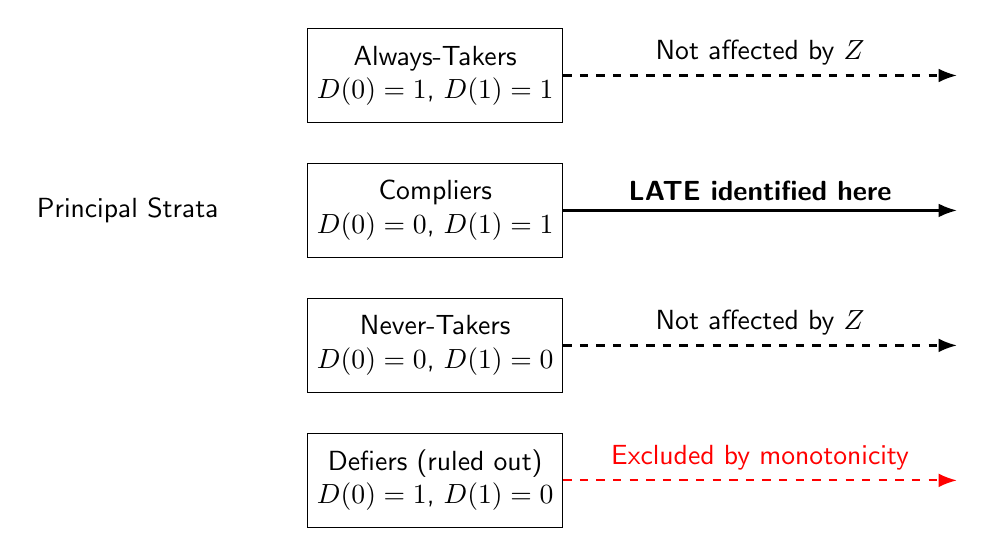
\begin{tikzpicture}[
    node distance=.5cm and 2cm,
    box/.style={rectangle, draw, minimum width=2.5cm, minimum height=1.2cm, align=center},
    arrow/.style={-{Latex}, thick}
]

% Boxes
\node[box] (at) {Always-Takers \\ $D(0) = 1$, $D(1) = 1$};
\node[box, below=of at] (c) {Compliers \\ $D(0) = 0$, $D(1) = 1$};
\node[box, below=of c] (nt) {Never-Takers \\ $D(0) = 0$, $D(1) = 0$};
\node[box, below=of nt] (d) {Defiers (ruled out) \\ $D(0) = 1$, $D(1) = 0$};

% Labels
\node[left=1cm of c, align=center] {Principal Strata};

% Arrows for explanation
\draw[arrow] (c.east) -- ++(5,0) node[midway, above] {\textbf{LATE identified here}};
\draw[arrow, dashed] (at.east) -- ++(5,0) node[midway, above] {Not affected by $Z$};
\draw[arrow, dashed] (nt.east) -- ++(5,0) node[midway, above] {Not affected by $Z$};
\draw[arrow, red, dashed] (d.east) -- ++(5,0) node[midway, above] {Excluded by monotonicity};

\end{tikzpicture}
\end{frame}


\begin{frame}{Who Are the Compliers? What Are Their Gains?}
\begin{itemize}
    \item In the model of heterogeneous returns to education:
    \[
    \beta_i = \gamma + v_{i}, \quad \text{where } v_{i} \text{ captures individual-specific deviations}
    \]

    \item The IV estimator identifies:
    \[
    \mathbb{E}[\beta_i\mid \text{Compliers}] = \gamma + \mathbb{E}[v_{i} \mid \text{Compliers}]
    \]

    \item \textbf{Who are the compliers?}
    \begin{itemize}
        \item Individuals whose educational choices are influenced by the instrument \( z_i \)
        \item They are at the \emph{margin of attending college}: those who attend if and only if encouraged
    \end{itemize}

    \item \textbf{What are their gains?}
    \begin{itemize}
        \item Depends on the relationship between the instrument and \( v_{i} \)
        \item If those at the margin have lower motivation, preparation, or ability, then:
        \[
        \mathbb{E}[v_{i1} \mid \text{Compliers}] < 0 \quad \Rightarrow \quad \text{LATE} < \text{ATE}
        \]
    \end{itemize}

    \item \textbf{Conclusion:} IV estimates are local — their policy relevance depends on \emph{who the compliers are}, and what their unobserved gains \( v_{i} \) look like.
\end{itemize}
\end{frame}


\section{IV weaknesses}

\begin{frame}{Challenges with IV}
\begin{itemize}
\item The IV estimator is among the most common tools of econometrics.
\item However, it has several weaknesses.
\begin{itemize}
\item Imprecision
\item Small sample Bias
\item Sensitivity to Weak Instruments
\end{itemize}
\end{itemize}
\end{frame}


\begin{frame}{Problems with IV estimator: Imprecision}
\begin{itemize}
\item Suppose Z and X are mean 0, $y=X\beta+e$,
\begin{align*}
Z'X&=X'Z=\sum z_ix_i=n*cov(z,x)\\\pause
Z'Z&=\sum z_i^2=n*var(z)\\\pause
X'X&=\sum x_i^2=n*var(x)\\\pause
\hat{\beta}_{IV}&=(Z'X)^{-1}Z'y\\\pause
\hat{\beta}_{OLS}&=(X'X)^{-1}X'y\\\pause
Avar(\hat{\beta}_{OLS})&=\sigma_e^2(X'X)^{-1}\\\pause
Avar(\hat{\beta}_{IV})&=\sigma_e^2(Z'X)^{-1}Z'Z(X'Z)^{-1}
\end{align*}
\end{itemize}
\end{frame}

\begin{frame}{Problems with IV estimator: Imprecision}
\begin{align*}
Avar(\hat{\beta}_{OLS})&=\sigma_e^2(X'X)^{-1}=\frac{\sigma_e^2}{n}\frac{1}{var(x)}\\\pause
Avar(\hat{\beta}_{IV})&=\sigma_e^2(Z'X)^{-1}Z'Z(X'Z)^{-1}=\frac{\sigma_e^2}{n^2}\frac{n*var(z)}{cov(x,z)^2}\\\pause
&=\frac{\sigma_e^2}{n}\frac{1}{var(x)}\frac{var(x)var(z)}{cov(x,z)^2}\\\pause
&=\frac{\sigma_e^2}{n}\frac{1}{var(x)}\frac{1}{\rho^2_{xz}}\\\pause
&=Avar(\hat{\beta}_{OLS})\frac{1}{\rho^2_{xz}}
\end{align*}
\begin{itemize}
\item As $\rho^2_{xz}\rightarrow 0$, $Avar(\hat{\beta}_{IV})\rightarrow \infty$
\end{itemize}
\end{frame}


\begin{frame}{Problems with IV estimator: Bias}
\begin{itemize}
\item IV is often is neither biased nor unbiased because it does not even have an expectation.
\item Kiviet has shown that the IV estimator has M moments, the number of overidentifying restrictions.  If $q=0$, IV has no expectation.
\end{itemize}
\begin{align*}
y&=X\beta+e\\
X&=Z\pi+v\\
\hat{\beta}_{IV}&=(X'P_ZX)^{-1}X'P_zy\\\pause
&=\beta+(X'P_ZX)^{-1}X'P_ze\\\pause
&=\beta+(X'P_ZX)^{-1}(\pi'Z'+v')P_ze\\\pause
&=\beta+(X'P_ZX)^{-1}(\pi'Z'+v')P_ze\\\pause
&=\beta+(X'P_ZX)^{-1}\pi'Z'P_ze+(X'P_ZX)^{-1}v'P_ze\\\pause
&=\beta+(X'P_ZX)^{-1}\pi'Z'e+(X'P_ZX)^{-1}v'P_ze
\end{align*}
\end{frame}



\begin{frame}{Form of small sample bias}
\begin{align*}
E(\hat{\beta}_{IV})-\beta&\approx E(X'P_ZX)^{-1}E(\pi'Z'e)+E(X'P_ZX)^{-1}E(v'P_ze)\\\pause
&=E(X'P_ZX)^{-1}\pi'E(Z'e)+E(X'P_ZX)^{-1}E(v'P_ze)\\\pause
&=(E(X'P_ZX))^{-1}E(v'P_ze)\\\pause
&=(E(\pi'Z'+v')P_z(Z\pi+v)))^{-1}E(v'P_ze)\\\pause
&=(E(\pi'Z'Z\pi+\pi'Z'v+v'Z\pi+v'P_zv))^{-1}E(v'P_ze)\\\pause
&=(E(\pi'Z'Z\pi)+E(v'P_zv))^{-1}E(v'P_ze) \tag{b/c $E(Z'e)=E(Z'v)=0$}\\\pause
&=(E(\pi'Z'Z\pi)+\sigma_{v}^2p)^{-1}\sigma^2_{ev} p\\\pause
&=\frac{1}{\left(\frac{E(\pi'Z'Z\pi)/p}{\sigma^2_v}+1\right)}\frac{\sigma_{ev}^2}{\sigma_v^2}
\end{align*}
\end{frame}


\begin{frame}{F-test}
\begin{align*}
E(\hat{\beta}_{IV})-\beta&\approx \frac{1}{\left(\frac{E(\pi'Z'Z\pi)/p}{\sigma^2_v}+1\right)}\frac{\sigma_{ev}^2}{\sigma_v^2}
\approx \frac{1}{\left(1+F_{p,n-p}\right)}\frac{\sigma_{ev}^2}{\sigma_v^2}
\end{align*}
\begin{itemize}
\item F is the test where the null is that all instrument coefficients are 0.
\item The bias of IV only goes away if $F\rightarrow \infty$
\item The bias of IV is the OLS bias as $F\rightarrow 0$.
\item Adding useless instruments increases p, which decreases F and increases the bias.
\end{itemize}
\end{frame}

\begin{frame}{Weak instruments}
Suppose we have a single $x$ and a single instrument $z$.  An instrument is weak if $\rho_{zx}$ is small.

\begin{align*}
plim \hat{\beta}_{OLS}&=plim \frac{cov(x,y)}{var(x)}=plim \frac{cov(x,\alpha+\beta+e)}{var(x)}\\
 &=\beta+plim \frac{cov(x,e)}{var(x)}=\beta+plim \frac{cov(x,e)}{\sqrt{var(x)}\sqrt{var(e)}}\frac{\sqrt{var(e)}}{\sqrt{var(x)}}\\
  &=\beta+\rho_{xe}\frac{\sigma_e}{\sigma_x}\\
    \end{align*}
 \end{frame}
 
 \begin{frame}{Weak instruments}
Suppose we have a single $x$ and a single instrument $z$.  An instrument is weak if $\rho_{zx}$ is small.

\begin{align*}
  plim \hat{\beta}_{IV}&=plim \frac{cov(x,\alpha+\beta+e)}{cov(z,x)}\\
     &=\beta+plim \frac{cov(z,e)}{cov(z,x)}=\beta+plim \frac{\frac{cov(z,e)}{\sqrt{var(x)}\sqrt{var(e)}}}{\frac{cov(z,x)}{\sqrt{var(x)}\sqrt{var(z)}}}\frac{\sqrt{var(e)}}{\sqrt{var(x)}}\\
 &=\beta+\frac{\rho_{ze}}{\rho_{zx}}\frac{\sigma_e}{\sigma_x}\\
 &=\beta+\frac{\rho_{ze}}{\rho_{zx}\rho_{xe}}\rho_{xe}\frac{\sigma_e}{\sigma_x}=\beta+\frac{\rho_{ze}}{\rho_{zx}\rho_{xe}}ABias(\hat{\beta}_{OLS})
   \end{align*}
 \end{frame}
 
\begin{frame}{Weak/Bad instruments are worse than OLS}
$$\frac{ABias(\hat{\beta}_{OLS})}{ABias(\hat{\beta}_{IV})}>1\rightarrow \frac{\rho_{ze}}{\rho_{zx}\rho_{xe}}> 1$$
If $\frac{\rho_{ze}}{\rho_{zx}\rho_{xe}}\geq 1$, then IV is more biased than OLS. \\

Suppose $\rho_{xu}=.5$, so X is super endogenous, $Z$ is barely endogenous: $\rho_{zu}=0.01$.\\
Small $\rho_{zx}=0.019$ gives $\frac{ABias(\hat{\beta}_{OLS})}{ABias(\hat{\beta}_{IV})}=1.052$.
\end{frame}

\begin{frame}{Testing power of instruments}
$$\frac{ABias(\hat{\beta}_{OLS})}{ABias(\hat{\beta}_{IV})}\approx \frac{1}{F}$$
F statistic of 100 means IV is 1\% as biased as OLS.
\end{frame}

\begin{frame}{Testing endogeneity via Durbin-Hausman-Wu test}
\begin{itemize}
\item If X is exogenous, then both OLS and IV are consistent, but OLS is BLUE.
\item Asymptotically, the difference between OLS and IV should converge to zero.
$$H=(\hat{\beta}_{IV}-\hat{\beta}_{OLS})'[Avar(\hat{\beta}_{IV})-Avar(\hat{\beta}_{OLS})]^{-1}(\hat{\beta}_{IV}-\hat{\beta}_{OLS})\sim \chi^2_{dim(\beta)}$$
\item Rejecting null says that OLS and IV are not close to one another, so either X is endogneous or Z is an invalid instrument. 
\end{itemize}
\end{frame}


\section{Heckman selection}

\begin{frame}{Heckman Selection}
\begin{itemize}
\item IV estimates the LATE under fairly reasonable assumptions.
\item Under stronger distributional assumptions we can get the ATE and the ATT.
$$\begin{pmatrix} u_i^1\\u_i^0\\e_i\end{pmatrix}\sim N\begin{pmatrix}\begin{pmatrix}0\\0\\0\end{pmatrix}, \begin{bmatrix}\sigma_1^2&\sigma_{01}&\sigma_{1e}\\ & \sigma^2_0&\sigma_{0e}\\&&1\end{bmatrix}\end{pmatrix}$$
\end{itemize}
\end{frame}

\begin{frame}{Conditional Expectations of Joint Normals}
Consider two jointly normal random variables $(X,Y)$.
$$
\begin{pmatrix} X \\ Y \end{pmatrix} \sim N\left(\begin{pmatrix}0 \\ 0\end{pmatrix}, \begin{pmatrix}\sigma_X^2 & \sigma_{XY} \\ \sigma_{XY} & \sigma_Y^2\end{pmatrix}\right)
$$

Then, the conditional expectation of $X$ given $Y > c$ is:

$$
E[X \mid Y > c] = \frac{\text{Cov}(X,Y)}{\sqrt{\text{Var}(Y)}} \cdot \frac{\phi\left(\frac{c}{\sqrt{\text{Var}(Y)}}\right)}{1-\Phi\left(\frac{c}{\sqrt{\text{Var}(Y)}}\right)}
$$

Here, $\phi(\cdot)$ and $\Phi(\cdot)$ are the PDF and CDF of the standard normal distribution, respectively.
\end{frame}

\begin{frame}{Application to Selection Model}

We focus on deriving:

$$
E[u_i^1 \mid e_i > -Z_i'\gamma]
$$

Using the previous result with $X=u_i^1$, $Y=e_i$, and threshold $c=-Z_i'\gamma$:

$$
E[u_i^1\mid e_i>-Z_i'\gamma] = \sigma_{1e}\frac{\phi(Z_i'\gamma)}{\Phi(Z_i'\gamma)}
$$


$$
E[u_i^0 \mid e_i < -Z_i'\gamma]
$$

$$
E[u_i^0\mid e_i<-Z_i'\gamma] = -\sigma_{1e}\frac{\phi(Z_i'\gamma)}{1-\Phi(Z_i'\gamma)}
$$
\end{frame}


\begin{frame}{Inverse Mills Ratio}
Define the \textbf{Inverse Mills Ratio} $\lambda(\cdot)$ as:

$$
\lambda(Z_i'\gamma) = \frac{\phi(Z_i'\gamma)}{\Phi(Z_i'\gamma)}
$$

Thus, the conditional expectation is:

$$
E[u_i^1\mid e_i>-Z_i'\gamma]=\sigma_{1e}\lambda(Z_i'\gamma)
$$

\begin{itemize}
\item $\sigma_{1e}$ captures correlation between selection and outcome errors.
\item $\lambda(Z_i'\gamma)$ measures the intensity of selection at given values of the selection index $Z_i'\gamma$.
\item We estimate $\gamma$ with a probit.
\end{itemize}

\end{frame}


\end{document}

